\documentclass[a4paper,12pt]{report}
\usepackage[utf8]{inputenc}
\usepackage{imakeidx}
\usepackage{graphicx}
\usepackage{float} %required for the placement specifier H
\usepackage{multicol}		%multicolumns
\usepackage{tabto}
\usepackage{listings}
\usepackage{comment}

\usepackage{color}

\definecolor{dkgreen}{rgb}{0,0.6,0}
\definecolor{gray}{rgb}{0.5,0.5,0.5}
\definecolor{mauve}{rgb}{0.58,0,0.82}

\lstset{frame=tb,
  language=Java,
  aboveskip=3mm,
  belowskip=3mm,
  showstringspaces=false,
  columns=flexible,
  basicstyle={\small\ttfamily},
  numbers=none,
  numberstyle=\tiny\color{gray},
  keywordstyle=\color{blue},
  commentstyle=\color{dkgreen},
  stringstyle=\color{mauve},
  breaklines=true,
  breakatwhitespace=true,
  tabsize=3
}

\makeindex[columns=3]

\pagenumbering{roman}

%opening
\title{WolfSSL}
\author{Luca Valentini}
\date{Insert Date}

\begin{document}
\maketitle
\tableofcontents



\newpage
\begin{abstract}
This document is meant to be a small introductory guide to wolfssl.
\\For the creation of this thesis I used the official wolfssl manual and some github repository related to wolfssl.
\end{abstract}


\pagenumbering{arabic}
\chapter{SSL Protocol}

\section{Introduction}
The SSL protool is a client/server protocol that provides the following basic security services to the communicating peers:
\begin{itemize}
	\item Authentication (both peer entity anda data origin authentication) services
	\item Connection confidentiality services
	\item Connection integrity services
\end{itemize}

The SSL protocol is sockets-oriented, meaning that all or none of the data that is sent to or received from a network connection is cryptographically protected in exactly the same way. It can be best viewed as an intermediate layer between the transporrt and the application layer that serves two purposes:
\begin{itemize}
	\item Establish a secure connection between the commucating peers
	\item Use this connection to securely trasmit giher-layer protocol data from the sender to the reciever. It therefore fragments the data in pieces called fragments; each fragment is optionally compressed, authenticated, encrypted, prepended with a header, and transmitted to the reciever. Each data fragment prepared this way is sent in a distinct SSL record.
\end{itemize}

\begin{figure}[H]
    \centering
    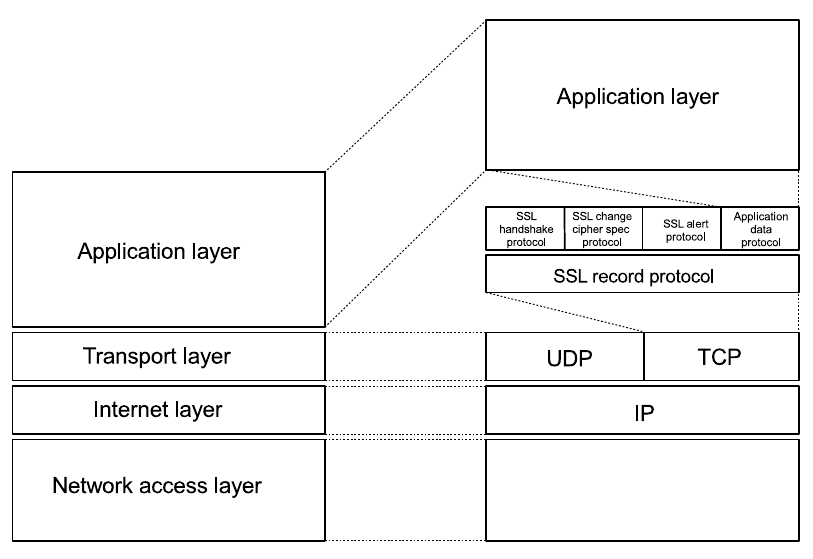
\includegraphics[scale=0.5]{subLayer_subProtocols.png}
    \caption{The SSL with its (sub)layer and (sub)protocols}
    \label{fig:galaxy}
\end{figure}

The SSL consists of two sublayers and a few subprotocols:
\begin{itemize}
	\item The lower sublayer is stacked on top of some connection-oriented and reliable transport layer protocol. This layer basically comprises the SSL record protocol that is used for the encapsulation of the higher-layer protocol data.
	\item The higher sublayer is stacked on top of the SSL record protocol and comprises four subprotocols.

	\begin{itemize}
		\item The \emph{SSL handshake protocol} is the core subprotocol of SSL. It is used for establishment of a secure connection. It allows the communicating peers to authenticate each other and to negotiate a cipher suite and a compression method.
		\item The \emph{SSL change cipher spec protocol} is used to put the parameters, set by the SSL handshake protocol in place and make them effective.
		\item The \emph{SSL alert protocol} allows the communicating peers to signal indicators of potential problems and send respective alert messages to each other.
		\item The \emph{SSL application data protocol} is used for the secure transmission of application data.
	\end{itemize}

\end{itemize}

In spite of the fact that SSL consists of several subprotocols, we use the term \emph{SSL protocol} to refer to all of them simultaneously.

\section{SSL Handshake}
The SSL handshake protocol is layered on top of the SSL record protocol. It allows a client and server to authenticate each other and to negotiate issues like cipher suites and compression methods.

\begin{figure}[H]
    \centering
    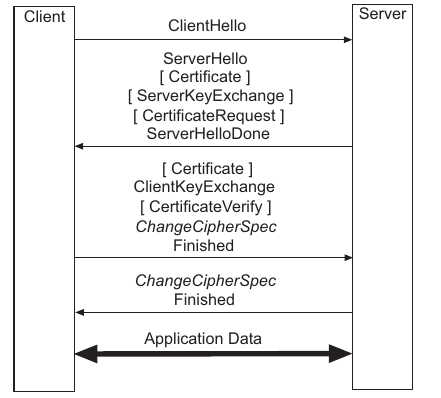
\includegraphics[scale=0.7]{handshake.png}
    \caption{The SSL handshake protocol}
    \label{fig:galaxy}
\end{figure}

\vspace{5mm} %5mm vertical space
The SSL handshake protocol comprises four sets of messages:
\begin{itemize}
\item The first flight comprises a single \emph{ClientHello} message that is sent from the client to the server.
\item The second flight comprises two messages that are sent back from the server to the client:
\begin{enumerate}
\item \emph{ServerHello} message is sent in response to the \emph{ClientHello} message
\item (optional) If the server is to authenticate itself, it may send a \emph{Certificate} message to the client.
\item (optional) Under some circumstances, the server may send a \emph{ServerKeyExchange} message to the client.
\item (optional) If the server requires the client to authenticate itself with a public key certificate, then it may send a \emph{CertificateRequest} message to the client.
\item Finally, server send a \emph{ServerHelloDone} message to the client.
\end{enumerate}
\item The third flight comprises three to five messages that are again sent from the client to the server:
\begin{enumerate}
\item (optional) If the server has sent a \emph{CertificateRequest} message, then the client sends a \emph{Certificate} message to the server.
\item In the main step of the protocol, the client sends a \emph{ClientKeyExchange} message to the server.
\item (optional) If the client has sent a certificate to the server, then it must also send a \emph{CertificateVerify} message to the server. This message is digitally signed with the private key that corresponds to the client certificate's public key.
\item The client sends a \emph{ChangeCipherSpec} message to the server (using the SSL change cipher spec protocol) and copies its pending write state into the current write state.
\item The client sends a \emph{Finished} message to the server. As mentioned above, this is the first message that is cryptographically protected under the new cipher spec.
\end{enumerate}
\item The fourth flight comprises two messages that are sent from the server back to the client:
\begin{enumerate}
\item The server sends another \emph{ChangeCipherSpec} message to the client and copies its pending write state into the current write state.
\item Finally, the server send a \emph{Finished} message to the client. Again, this message is cryptographically protected under the new cipher spec.

\end{enumerate}
\end{itemize}

At this point in time, the SSL handshake is complete and the client and server may start exchanging application-layer data.

\chapter{WolfSSL}
The wolfSSL embedded SSL library is a lightweight SSL/TLS library written in ANSI C and targeted for embedded, RTOS, and resource-constrained
environments - primarily because of its small size, speed, and feature set; It's an SSL/TLS library optimized to run on embedded platforms.
\\It's free and it has an excellent cross platform support.
\\WolfSSL supports standards up to the current TLS 1.3 and DTLS 1.2 levels, is up to
20 times smaller than OpenSSL and it's powered by the colfCrypt library.

\vspace{5mm} %5mm vertical space
This library is built for maximum portability and supports the C programming language as a primary interface. It also supports several other host languages, including Java (wolfSSL JNI), C\# (wolfSSL C\#), Python, and PHP and Perl.

\vspace{5mm} %5mm vertical space
To improve performance it supports hardware cryptography and acceleration on several platforms.

\vspace{5mm} %5mm vertical space
In the following list you can see some of WolfSSI’s features:
\begin{itemize}
\item Runtime memory usage between 1-36 kB
\item OpenSSl compatibility layer
\item Hash Functions: \begin{multicols}{3}\begin{itemize}
\item MD2
\item MD4
\item MD5
\item SHA-1
\item SHA-224
\item SHA-256
\item SHA-384
\item SHA-512
\item BLAKE2b
\item RIPEMD-160
\item Poly1305
\end{itemize}
\end{multicols}
\item Mutual authentication support (client/server)
\item SSL Sniffer (SSL Inspection) Support
\item IPv4 and IPv6 support


\end{itemize}

\cleardoublepage
The operating systems supported are:
\begin{multicols}{3}
\begin{enumerate}
\item Win32/64 \item Linux \item Mac OS X \item Solaris \item ThreadX \item VxWorks \item FreeBSD \item NetBSD \item OpenBSD \item embedded Linux \item Yocto Linux \item OpenEmbedded \item WinCE \item Haiku \item OpenWRT \item iPhone(iOS) \item Android \item Nintendo Wii and Gamecube through DevKitPro \item QNX \item MontaVista \item NonStop \item TRON / ITRON /  ITRON \item Micrium  C / OS - III \item FreeRTOS \item SafeRTOS \item NXP / Freescale MQX \item Nucleus \item TinyOS \item HP / UX \item AIX \item ARC MQX \item TI - RTOS \item uTasker \item embOS \item INtime \item Mbed \item uT - Kernel \item RIOT \item CMSIS -RTOS \item FROSTED \item Green Hills INTEGRITY \item Keil RTX \item TOPPERS \item PetaLinux \item Apache Mynewt \item PikeOS 
\end{enumerate}
\end{multicols}

\chapter{Test case}
\section{Client/Server provided by WolSSL}

\begin{figure}[H]
    \centering
    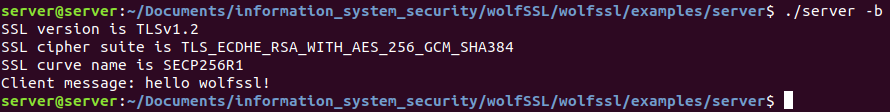
\includegraphics[scale=0.5]{test/examples/client-server/server.png}
    \caption{Server SSL}
    \label{fig:galaxy}
\end{figure}

\begin{figure}[H]+
    \centering
    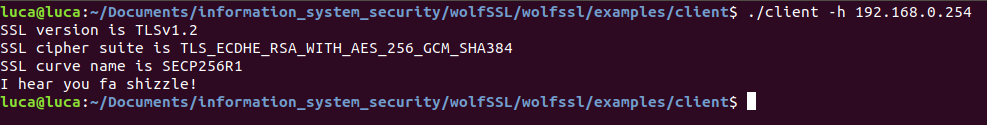
\includegraphics[scale=0.45]{test/examples/client-server/client.png}
    \caption{Client SSL}
    \label{fig:galaxy}
\end{figure}

In this example, the server is a simple SSL server that allows only one client connection; after the connection with a client, the server receives an encrypted message from client, it responds and quits.
\\The -b parameter allows the server to bind to any interface instead of localhost only.
\\
\\The client after the connection with the server, sends a message (hello wolfssl!) and after the server response, it quits.
\\The -h parameter allows the client to specify the server address to perform the connection.

\begin{figure}[H]
    \centering
    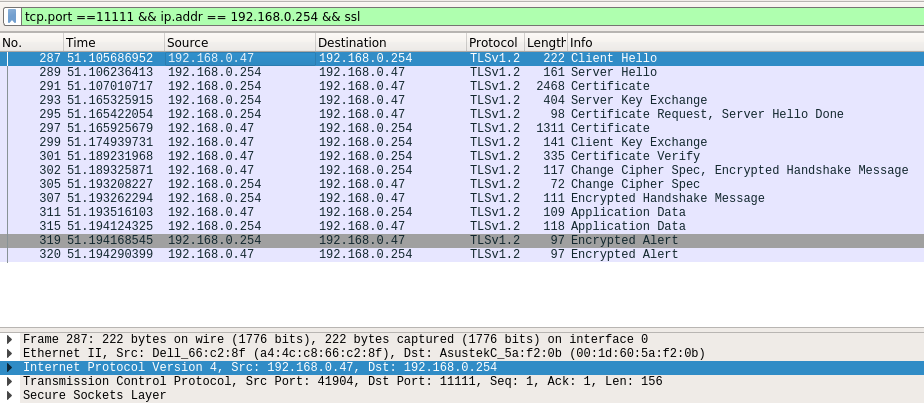
\includegraphics[scale=0.5]{test/examples/client-server/wireshark1.png}
    \caption{All SSL packets sent}
    \label{fig:galaxy}
\end{figure}
Client IP:  192.168.0.47 \hspace{4cm} Server IP: 192.168.0.254\\ \\
Come si puo' bene vedere dalla figura soprastante, la comunicazione viene iniziata dal client con un 'Client Hello'; dopo SSL handshake, ci sono due messaggi 'Application Data' inviati rispettivamente dal client verso il server e dal server verso il client il cui contenuto e' cifrato. Una volta che il server invia la risposta al client, la comunicazione viene chiusa attraverso 'Encrypted Alert'.

\begin{figure}[H]
    \centering
    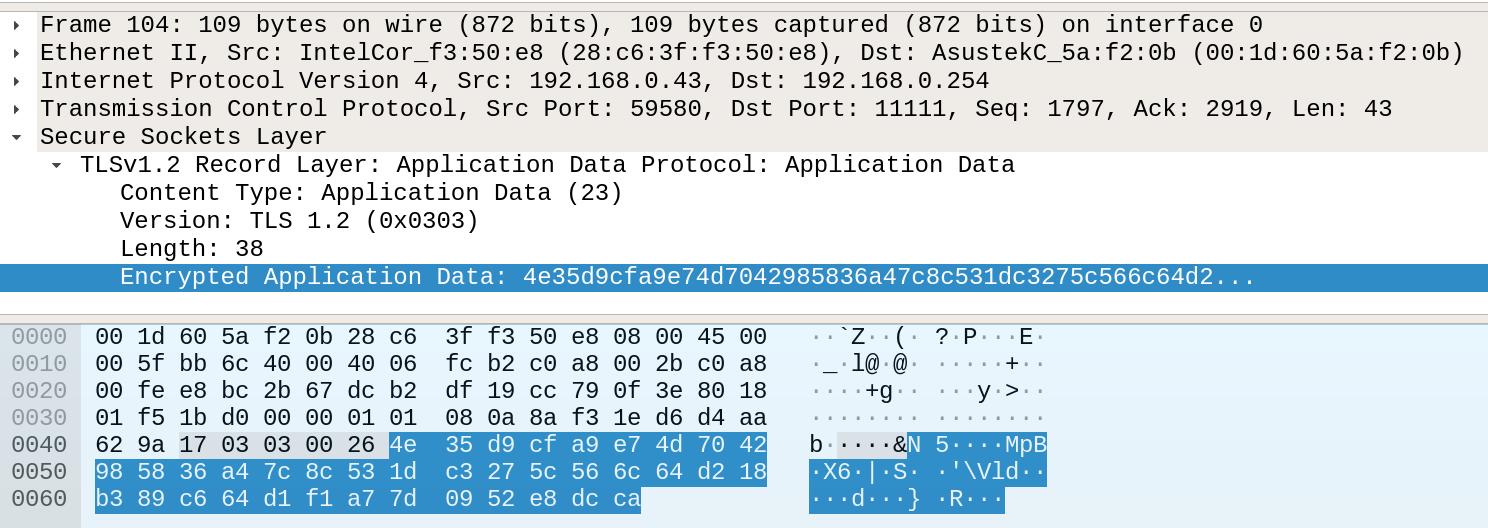
\includegraphics[scale=0.3]{test/examples/client-server/encrypted_data.png}
    \caption{Content of the encrypted message}
    \label{fig:galaxy}
\end{figure}

Come si puo' vedere, lo scambio di messaggi e' cifrato.


\pagebreak

\section{EchoClient/EchoServer provided by WolfSSL}
\begin{figure}[H]
\hspace*{-1cm}     
    \centering
    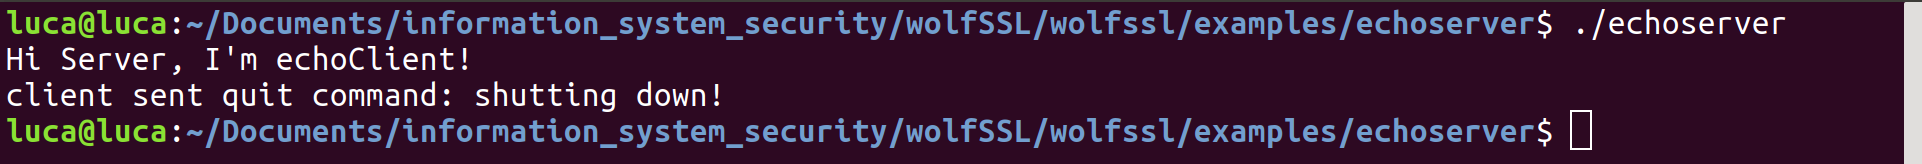
\includegraphics[scale=0.25]{test/examples/echoclient-echoserver/echoServer.png}
    \caption{EchoServer SSL}
    \label{fig:galaxy}
\end{figure}

\begin{figure}[H]
\hspace*{-1cm}     
    \centering
    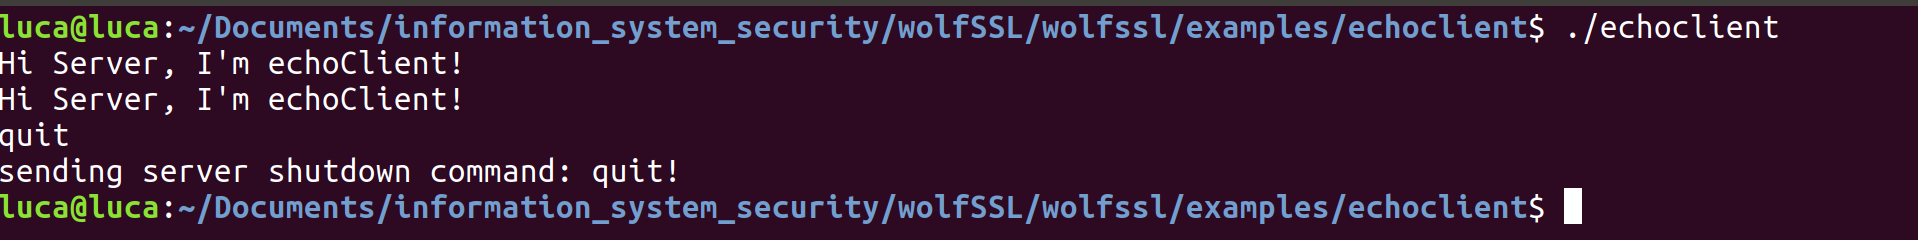
\includegraphics[scale=0.25]{test/examples/echoclient-echoserver/echoClient.png}
    \caption{EchoClient SSL}
    \label{fig:galaxy}
\end{figure}

\begin{figure}[H]
\hspace*{-2cm}     
    \centering
    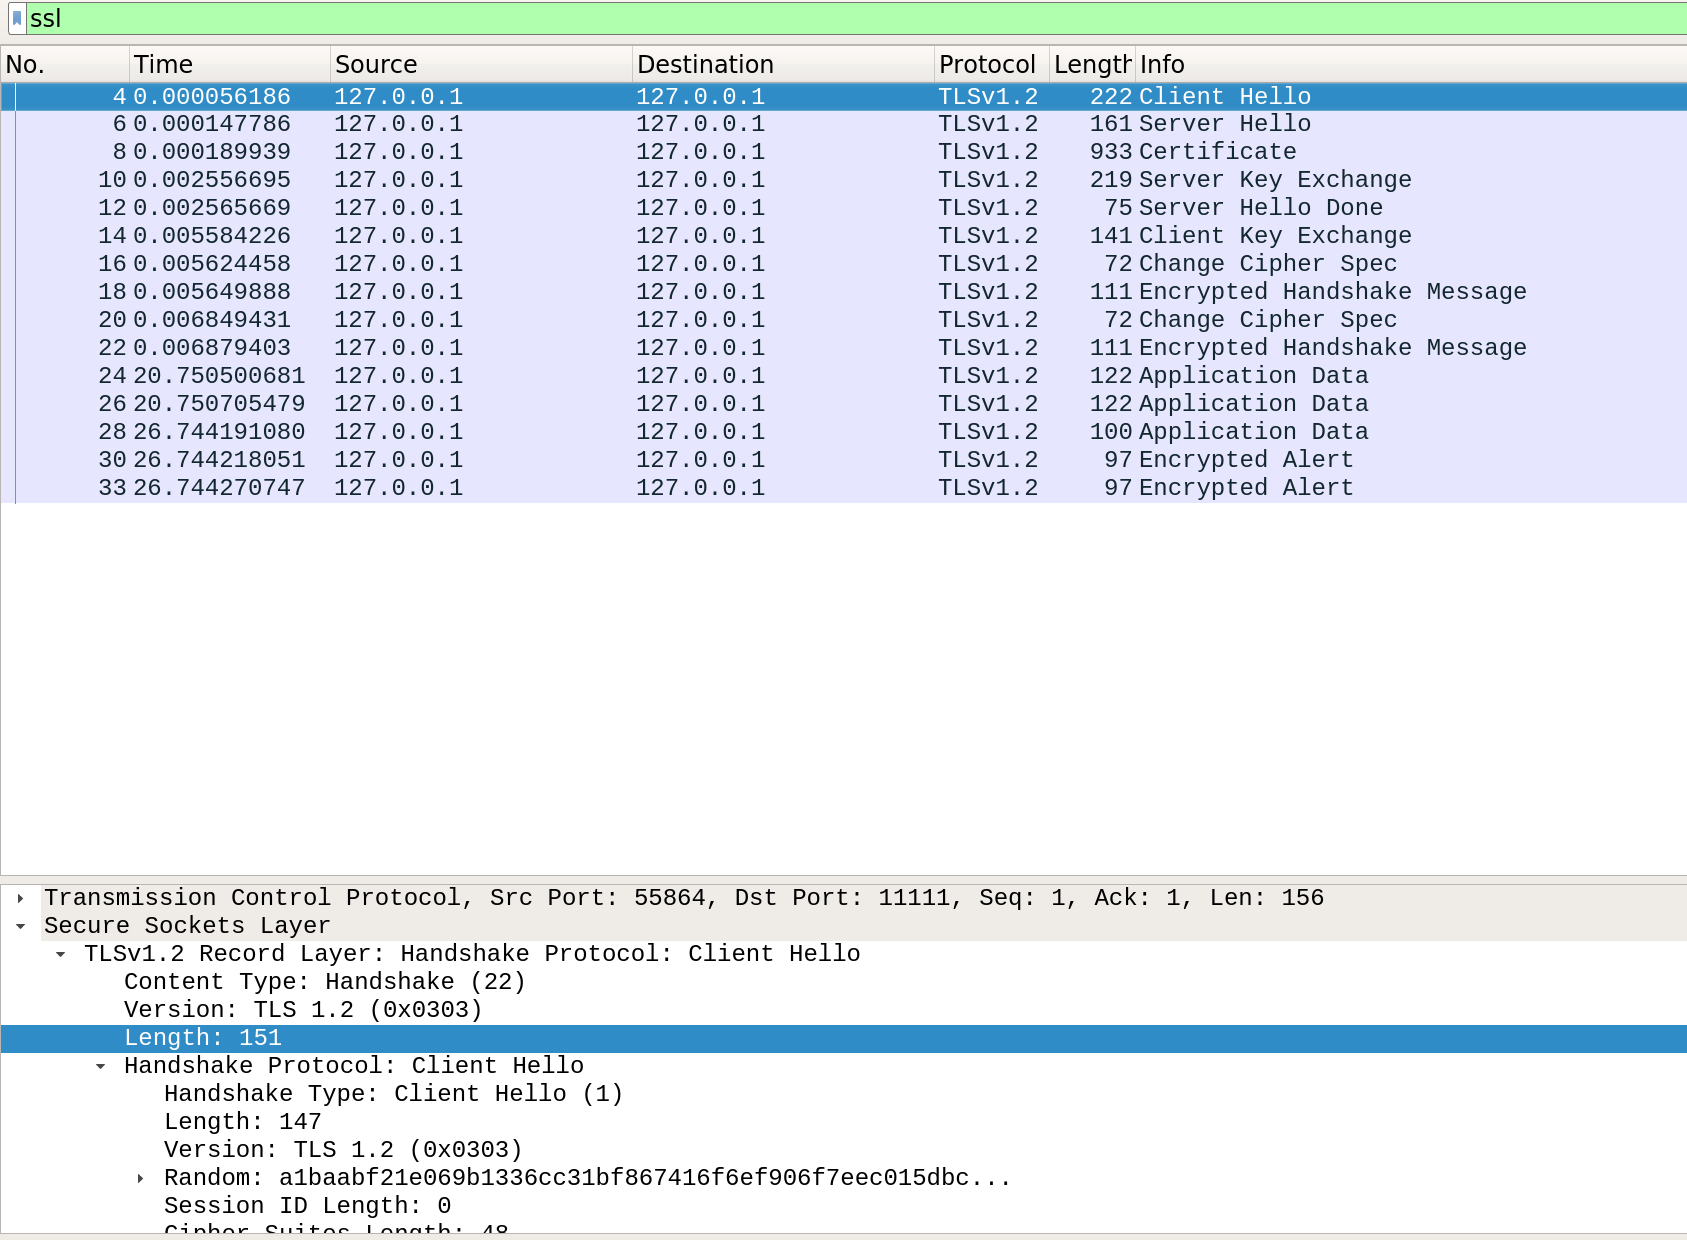
\includegraphics[scale=0.3]{test/examples/echoclient-echoserver/wireshark.png}
    \caption{All SSL packets sent}
    \label{fig:galaxy}
\end{figure}

\chapter{Create a program using WolfSSL}
\section{TCP application}
To create an SSL program you can modify your TCP program added several SSL functions. To explain the migration from TCP to SSL, I created a simple chat between a client and a server available on github.
\begin{comment}
\subsection{TCP Server}

In my example, the TCP server after configuring the socket and connecting it with the client, it creates a ClientHandler thread that launches a thread for read and a thread for write from socket.
\begin{lstlisting}[caption={int main() of TCP server},captionpos=b][language=c]

int main()
{
    /* Create a socket that uses an internet IPv4 address,
     * Sets the socket to be stream based (TCP),
     * 0 means choose the default protocol. */
    if ((sockfd = socket(AF_INET, SOCK_STREAM, 0)) == -1)
    {
        fprintf(stderr, "ERROR: failed to create the socket\n");
        return -1;
    }

    /* Initialize the server address struct with zeros */
    memset(&servAddr, 0, sizeof(servAddr));

    /* Fill in the server address */
    servAddr.sin_family = AF_INET;           /* using IPv4      */
    servAddr.sin_port = htons(DEFAULT_PORT); /* on DEFAULT_PORT */
    servAddr.sin_addr.s_addr = INADDR_ANY;   /* from anywhere   */

    /* Bind the server socket to our port */
    if (bind(sockfd, (struct sockaddr *)&servAddr, sizeof(servAddr)) == -1)
    {
        fprintf(stderr, "ERROR: failed to bind\n");
        return -1;
    }

    /* Listen for a new connection*/
    if (listen(sockfd, 1) == -1)
    {
        fprintf(stderr, "ERROR: failed to listen\n");
        return -1;
    }
    /* Continue to accept clients until shutdown is issued */
    while (1)
    {
        printf("Waiting for a connection...\n");
        /* Accept client connections */
        if ((connd = accept(sockfd, (struct sockaddr *)&clientAddr, &size)) == -1)
        {
            fprintf(stderr, "ERROR: failed to accept the connection\n\n");
            ncurses_end();
            return -1;
        }
        pthread_t mainThread;
        pthread_create(&mainThread, NULL, ClientHandler, NULL);
        pthread_join(mainThread, NULL);
        printText("Communication is ended!\n", "System");

        if (is_end)
            break;
    }
    ncurses_end();
    printf("Shutdown complete\n");

    /* Cleanup after this connection */
    close(connd); /* Close the connection to the client   */
    /* Cleanup and return */
    close(sockfd); /* Close the socket listening for clients   */
    return 0;      /* Return reporting a success               */
}

\end{lstlisting}

As stated above, the clientHandler thread creates two thread, but before it waits the client username.

\begin{lstlisting}[caption={clientHandler thread of TCP server},captionpos=b][language=c]
void *ClientHandler(void *args)
{
    int ret;
    /*********************** USERNAME */
    /* Read the client username into our buff array */
    XMEMSET(buff, 0, sizeof(buff));
    ret = read(connd, buff, sizeof(buff));
    ncurses_start();
    clearWin();
    if (ret > 0)
    {
        /* Print to stdout any data the client sends */
        strcpy(username, buff);
        char text[256];
        sprintf(text, "Client %s connected successfully", username);
        printText(text, "System");
        printText("***************************\n", "System");
        fflush(stdout);
    }
    else
    {
        printText("ERROR!!", "System");
        close(sockfd);      /* Close the connection to the server   */
        pthread_exit(NULL); /* End theread execution                */
    }
    /****************************    */
    XMEMSET(buff, 0, sizeof(buff));

    if (pthread_create(&Treader, NULL, readBuffer, NULL))
    {
        fprintf(stderr, "Error creating thread\n");
        fflush(stdout);
        return NULL;
    }

    if (pthread_create(&Twriter, NULL, writeBuffer, NULL))
    {
        fprintf(stderr, "Error creating thread\n");
        fflush(stdout);
        return NULL;
    }
    pthread_join(Treader, NULL);
    pthread_join(Twriter, NULL);
    /* Cleanup after this connection */
    close(connd);       /* Close the connection to the client   */
    pthread_exit(NULL); /* End theread execution                */
}

\end{lstlisting}


ReadBuffer is a thread that allows to read messages sent from client. It has an infinite loop that read data from socket open previously; Once it gets the message, with the printText function, the message is printed to the terminal using ncurses. 
\begin{lstlisting}[caption={readBuffer thread of TCP server},captionpos=b][language=c]
void *readBuffer(void *args)
{
    int ret;
    while (1)
    {
        /* Read the client data into our buff array */
        XMEMSET(buffReader, 0, sizeof(buffReader));
        ret = read(connd, buffReader, sizeof(buffReader));

        if (ret > 0)
        {
            if (!strcmp(buffReader, "quit"))
            {
                pthread_cancel(Twriter);
                pthread_exit(NULL); /* End threaded execution                */
            }
            printText(buffReader, username);
        }
        else
        {
            printText("ERROR READ!!", "System");
            pthread_cancel(Twriter);
            pthread_exit(NULL); /* End threaded execution                */
        }
    }
}

\end{lstlisting}
WriteBuffer thread has an infinite loop used for write messages from server to client.
\begin{lstlisting}[caption={writeBuffer thread of TCP server},captionpos=b][language=c]
void *writeBuffer(void *args)
{
    int ret;
    while (1)
    {
        read_in();
        len = XSTRLEN(Rbuffer);

        /* Reply back to the client */
        ret = write(connd, Rbuffer, len);
        printText(Rbuffer, "Server");

        if (XSTRNCMP(Rbuffer, "quit", 4) == 0)
        {
            is_end = 1;
            break;
        }

        if (ret != len)
        {
            printText("ERROR!!", "System");
            break;
        }
    }
    pthread_cancel(Treader);
    return NULL;
}

\end{lstlisting}
\pagebreak
\end{comment}
\section{From TCP to SSL}
To create a wolfSSL application the first thing that I did is include the wolfSSL API header in your program.
\begin{lstlisting}[language=c]
#include <wolfssl/ssl.h>
\end{lstlisting}
After the inclusion of the header files, I initialize the library and the WOLFSSL\_CTX calling \textbf{wolfSSL\_Init}; This is necessary to use the library.
\\\\ The WOLFSSL\_CTX structure contains global values for each SSL connection, including certificate information.
To create a new WOLFSSL\_CTX there is \textbf{wolfSSL\_CTX\_new()} function. it requires an argument which defines the SSL or TLS protocol for the client or server to use. In my case I used TLS 1.3, so the call is: 
\begin{lstlisting}[language=c]
WOLFSSL_CTX *ctx = wolfSSL_CTX_new(wolfTLSv1_3_server_method());
\end{lstlisting}
for the server;
\begin{lstlisting}[language=c]
WOLFSSL_CTX *ctx = wolfSSL_CTX_new(wolfTLSv1_3_client_method())
\end{lstlisting}
for the client.
\\\\In the WOLFSSL\_CTX can be loaded the CA (Certificate Authority) so that the client is able to verify the server's identity when they start the connection. To load the CA into the WOLFSSL\_CTX there is \\\textbf{wolfSSL\_CTX\_load\_verify\_locations()}. This function requires three arguments:
\begin{itemize}
\item a WOLFSSL\_CTX pointer
\item a certificate file
\item a path value that point to a directory which should contain CA certificates in PEM format.
\end{itemize}
this function returns SSL\_SUCCESS or SSL\_FAILURE.
\\\textbf{wolfSSL\_CTX\_load\_verify\_locations()} can be used for verify the client or the server identity, but in my case, only the client loads the CA, the server loads a certificate file into the SSL context (WOLFSSL\_CTX) calling:
\begin{lstlisting}[language=c]
int wolfSSL_CTX_use_certificate_file(ctx, CERT_FILE, SSL_FILETYPE_PEM);
\end{lstlisting}
Also the server private key can be loaded using the wolfSSL library; the function is:
\begin{lstlisting}[language=c]
int wolfSSL_CTX_use_PrivateKey_file(ctx, KEY_FILE, SSL_FILETYPE_PEM)
\end{lstlisting}

After a TCP connection the WOLFSSL object needs to be created and the file descriptor needs to be associated with the session; the instructions are:
\begin{lstlisting}[language=c]
//Connect to socket file descriptor
WOLFSSL* ssl;
//create WOLFSSL object
ssl = wolfSSL_new(ctx);
wolfSSL_set_fd(ssl,sockfd);
\end{lstlisting}
After the previous instructions called by client and server, the server waits an SSL client to initiate the SSL handshake; it waits until a client call \textbf{wolfSSL\_connect(ssl)} and then the handshake starts.
\\\\Once the connection functions are set, I replaced \textbf{read(...)} function with: 
\begin{lstlisting}[language=c]
int wolfSSL_read(WOLFSSL *ssl, void *data, int sz);
\end{lstlisting}
It read \textbf{sz} bytes from the SSL session \textbf{ssl} internal read buffer into the buffer \textbf{data}. The bytes are removed from the internal receive buffer;
\\\\Instead the \textbf{write(...)} function is replaced by:
\begin{lstlisting}[language=c]
int wolfSSL_write(WOLFSSL *ssl, void *data, int sz);
\end{lstlisting}
It writes \textbf{sz} bytes from the buffer, \textbf{data}, to the SSL connection, \textbf{ssl}.
\\\\When the application is over, the WOLFSSL\_CTX object and the wolfSSL library must be freed; the instructions are:
\begin{lstlisting}[language=c]
wolfSSL_free(ssl);
wolfSSL_CTX_free(ctx);
wolfSSL_Cleanup();
\end{lstlisting}

\pagebreak
\section{SSL application}
To develop an SSL application, I started from the TCP chat explained in the previous section and I added the wolfSSL function to create an encrypted communication.
\\The goal of this program is to show how to create a simple encrypted chat, focusing on the security of an application and not to the good practices of the socket and thread applications.
\\Some part of the code like inclusion and global variables are omitted (wolfSSL object and other variables are stored in global memory); you can find them on github.
\\In the next subsections I'll try to explain the code of the program:
\subsection{SSL Server}
The server created by me authenticate itself by sending a certificate; For testing purpose, all the certificates that I use, I took from wolfSSL download.
\\It also use an RSA key for secure symmetric key exchange that is used for actual transmitted data encryption and decryption.
\\After the initialization of the wolfSSL and the socket, the main function marks the socket referred to by sockfd as a passive socket, that is, as a socket that will be used to accept incoming connection requests using accept.
\begin{lstlisting}[caption={int main() of SSL server, 1* part},captionpos=b][language=c]
int main()
{
    int ret;

    /* Initialize wolfSSL */
    wolfSSL_Init();

    /* Create a socket that uses an internet IPv4 address,
     * Sets the socket to be stream based (TCP),
     * 0 means choose the default protocol. */
    if ((sockfd = socket(AF_INET, SOCK_STREAM, 0)) == -1)
    {
        fprintf(stderr, "ERROR: failed to create the socket\n");
        return -1;
    }
    /* Create and initialize WOLFSSL_CTX */
    
    if ((ctx = wolfSSL_CTX_new(wolfTLSv1_3_server_method())) == NULL)
    {
        fprintf(stderr, "ERROR: failed to create WOLFSSL_CTX\n");
        return -1;
    }

    /* Load server certificates into WOLFSSL_CTX */
    if (wolfSSL_CTX_use_certificate_file(ctx, CERT_FILE, SSL_FILETYPE_PEM) != SSL_SUCCESS)
    {
        fprintf(stderr, "ERROR: failed to load %s, please check the file.\n",
                CERT_FILE);
        return -1;
    }

    /* Load server key into WOLFSSL_CTX */
    if (wolfSSL_CTX_use_PrivateKey_file(ctx, KEY_FILE, SSL_FILETYPE_PEM) != SSL_SUCCESS)
    {
        fprintf(stderr, "ERROR: failed to load %s, please check the file.\n",
                KEY_FILE);
        return -1;
    }

    /* Initialize the server address struct with zeros */
    memset(&servAddr, 0, sizeof(servAddr));

    /* Fill in the server address */
    servAddr.sin_family = AF_INET;           /* using IPv4      */
    servAddr.sin_port = htons(DEFAULT_PORT); /* on DEFAULT_PORT */
    servAddr.sin_addr.s_addr = INADDR_ANY;   /* from anywhere   */

    /* Bind the server socket to our port */
    if (bind(sockfd, (struct sockaddr *)&servAddr, sizeof(servAddr)) == -1)
    {
        fprintf(stderr, "ERROR: failed to bind\n");
        return -1;
    }

    /* Listen for a new connection*/
    if (listen(sockfd, 1) == -1)
    {
        fprintf(stderr, "ERROR: failed to listen\n");
        return -1;
    }
   .
   .
   .
\end{lstlisting}
This server can communicate with one client at a time so there is an infinite loop where the encrypted connection with a client is established. At this point a mainThread is created to handle reading and writing through the secure channel. Whenever the connection falls, the thread ends and the server try to established a new connection. The server ends only when keyboard of the server type 'quit' (this part is in another function).
\begin{lstlisting}[caption={int main() of SSL server, 2* part},captionpos=b][language=c]
    /* Continue to accept clients until shutdown is issued */
    while (1)
    {
	    printf("Waiting for a connection...\n");
        /* Accept client connections */
        if ((connd = accept(sockfd, (struct sockaddr *)&clientAddr, &size)) == -1)
        {
            fprintf(stderr, "ERROR: failed to accept the connection\n\n");
            return -1;
        }

        /* Create a WOLFSSL object */
        if ((ssl = wolfSSL_new(ctx)) == NULL)
        {
            fprintf(stderr, "ERROR: failed to create WOLFSSL object\n");
            return -1;
        }

        /* Attach wolfSSL to the socket */
        wolfSSL_set_fd(ssl, connd);

        /* Establish TLS connection */
        ret = wolfSSL_accept(ssl);
        if (ret != SSL_SUCCESS)
        {
            fprintf(stderr, "wolfSSL_accept error = %d\n",
                    wolfSSL_get_error(ssl, ret));
            return -1;
        }

        printf("Client connected successfully\n");
        pthread_t mainThread;
        pthread_create(&mainThread, NULL, ClientHandler, NULL);
        pthread_join(mainThread, NULL);
        printText("Communication is ended!\n", "System");

        if (is_end)
            break;
    }
    ncurses_end();
    printf("Shutdown complete\n");

    /* Cleanup after this connection */
    wolfSSL_free(ssl); /* Free the wolfSSL object              */
    close(connd);      /* Close the connection to the client   */
    /* Cleanup and return */
    wolfSSL_CTX_free(ctx); /* Free the wolfSSL context object          */
    wolfSSL_Cleanup();     /* Cleanup the wolfSSL environment          */
    close(sockfd);         /* Close the socket listening for clients   */
    return 0;              /* Return reporting a success               */
}
\end{lstlisting}

The previously created thread executes ClientHandler function; even if the connection is established, it shows 'Client name connected successfully' message on the screen only after reading the username from the secure channel.
\\After that two thread are created, one for read messages and one for write messages.
\begin{lstlisting}[caption={ClientHandler() of SSL server},captionpos=b][language=c]
void *ClientHandler(void *args)
{
    int ret;
    /*********************** USERNAME */
    /* Read the client username into our buff array */
    XMEMSET(buff, 0, sizeof(buff));
    ret = wolfSSL_read(ssl, buff, sizeof(buff) - 1);
    ncurses_start();
    clearWin();
    if (ret > 0)
    {
        /* Print to stdout any data the client sends */
        strcpy(username, buff);
        char text[256];
        sprintf(text, "Client %s connected successfully", username);
        printText(text, "System");
        printText("***************************\n", "System");
        fflush(stdout);
    }
    else
    {
        printText("ERROR!!", "System");
        close(sockfd);      /* Close the connection to the server   */
        pthread_exit(NULL); /* End theread execution                */
    }
    /****************************    */
    XMEMSET(buff, 0, sizeof(buff));

    if (pthread_create(&Treader, NULL, readBuffer, NULL))
    {
        fprintf(stderr, "Error creating thread\n");
        fflush(stdout);
        return NULL;
    }

    if (pthread_create(&Twriter, NULL, writeBuffer, NULL))
    {
        fprintf(stderr, "Error creating thread\n");
        fflush(stdout);
        return NULL;
    }

    pthread_join(Treader, NULL);
    pthread_join(Twriter, NULL);
    /* Cleanup after this connection */
    close(connd);       /* Close the connection to the client   */
    pthread_exit(NULL); /* End theread execution                */
}

\end{lstlisting}
WriteBuffer is a function executes by a thread for writing in the channel. \textbf{read\_in()} read the characters typed from the user until a new line and then sent the message with \textbf{wolfSSL\_write(ssl,Rbuffer,len)}.
\begin{lstlisting}[caption={writeBuffer() of SSL server},captionpos=b][language=c]
void *writeBuffer(void *args)
{
    int ret;
    while (1)
    {
        read_in();
        len = XSTRLEN(Rbuffer);

        /* Reply back to the client */
        do
        {
            ret = wolfSSL_write(ssl, Rbuffer, len);
            /* TODO: Currently this thread can get stuck infinitely if client
         *       disconnects, add timer to abort on a timeout eventually,
         *       just an example for now so allow for possible stuck condition
         */
            printText(Rbuffer, "Server");

        } while (wolfSSL_want_write(ssl));

        if (XSTRNCMP(Rbuffer, "quit", 4) == 0)
        {
            is_end = 1;
            break;
        }

        if (ret != len)
        {
            printText("ERROR!!", "System");
            break;
        }
    }
    pthread_cancel(Treader);
    return NULL;
}
\end{lstlisting}
ReadBuffer function read messages from the channel through \textbf{wolfSSL\_read(ssl, buffReader, sizeof(buffReader)-1)}. If the user on the other side writes 'quit', this function and writeBuffer function end.
\begin{lstlisting}[caption={readBuffer() of SSL server},captionpos=b][language=c]
void *readBuffer(void *args)
{
    int ret;
    while (1)
    {
        /* Read the client data into our buff array */
        XMEMSET(buffReader, 0, sizeof(buffReader));
        ret = wolfSSL_read(ssl, buffReader, sizeof(buffReader) - 1);

        if (ret > 0)
        {
            if (!strcmp(buffReader, "quit"))
            {
                pthread_cancel(Twriter);
                pthread_exit(NULL); /* End theread execution                */
            }
            printText(buffReader, username);
        }
        else
        {
            printText("ERROR READ!!", "System");
            pthread_cancel(Twriter);
            pthread_exit(NULL); /* End theread execution                */
        }
    }
}
\end{lstlisting}
\pagebreak
\subsection{SSL Client}
The SSL client has 3 thread; The main thread called Tclient that is used to manage read and write threads.
\\To execute the SSL client, the program needs the IP address of server. If the user doesn't provide it during the program calls, the program ends. 
\begin{lstlisting}[caption={int main() of SSL client},captionpos=b][language=c]
int main(int argc, char **argv)
{
    pthread_t Tclient;
    /* Check for proper calling convention */
    if (argc != 2)
    {
        printf("usage: %s <IPv4 address>\n", argv[0]);
        return -1;
    }
    ip = argv[1];
    /* create a second thread which executes inc_x(&x) */
    if (pthread_create(&Tclient, NULL, client, NULL))
    {
        fprintf(stderr, "Error creating thread\n");
        fflush(stdout);
        return 1;
    }
    if (pthread_join(Tclient, NULL))
    {
        fprintf(stderr, "Error joining thread\n");
        return 2;
    }
    ncurses_end();
    return 0; /* Return reporting a success               */
}
\end{lstlisting}
As in the server part, the function below is executed by a thread; it initializes WOLFSSL objects, socket etc. After initializations the function tries to connect to the secure channel, through the IP address inserted at the execution of the client.
\begin{lstlisting}[caption={void *client(void *args) of SSL client},captionpos=b][language=c]
void *client(void *args)
{
    struct sockaddr_in servAddr;

    printf("Set your username: ");
    refresh();
    if (!scanf("%s", username))
    {
        fprintf(stderr, "ERROR: failed to get message for server\n");
        return NULL;
    }
    ncurses_start();
    /* Initialize wolfSSL */
    wolfSSL_Init();

    /* Create a socket that uses an internet IPv4 address,
     * Sets the socket to be stream based (TCP),
     * 0 means choose the default protocol. */
    if ((sockfd = socket(AF_INET, SOCK_STREAM, 0)) == -1)
    {
        fprintf(stderr, "ERROR: failed to create the socket\n");
        return NULL;
    }

    /* Create and initialize WOLFSSL_CTX */
    if ((ctx = wolfSSL_CTX_new(wolfTLSv1_3_client_method())) == NULL)
    {
        fprintf(stderr, "ERROR: failed to create WOLFSSL_CTX\n");
        return NULL;
    }

    /* Load client certificates into WOLFSSL_CTX */
    if (wolfSSL_CTX_load_verify_locations(ctx, CERT_FILE, NULL) != SSL_SUCCESS)
    {
        fprintf(stderr, "ERROR: failed to load %s, please check the file.\n",
                CERT_FILE);
        return NULL;
    }

    /* Initialize the server address struct with zeros */
    memset(&servAddr, 0, sizeof(servAddr));

    /* Fill in the server address */
    servAddr.sin_family = AF_INET;           /* using IPv4      */
    servAddr.sin_port = htons(DEFAULT_PORT); /* on DEFAULT_PORT */

    /* Get the server IPv4 address from the command line call */
    if (inet_pton(AF_INET, ip, &servAddr.sin_addr) != 1)
    {
        fprintf(stderr, "ERROR: invalid address\n");
        return NULL;
    }

    /* Connect to the server */

    if (connect(sockfd, (struct sockaddr *)&servAddr, sizeof(servAddr)) == -1)
    {
        printText("ERROR: failed to connect", "System");
        return NULL;
    }
    /*Do something*/

    /* Create a WOLFSSL object */
    if ((ssl = wolfSSL_new(ctx)) == NULL)
    {
        fprintf(stderr, "ERROR: failed to create WOLFSSL object\n");
        return NULL;
    }

    /* Attach wolfSSL to the socket */
    wolfSSL_set_fd(ssl, sockfd);
    /* Connect to wolfSSL on the server side */
    if (wolfSSL_connect(ssl) != SSL_SUCCESS)
    {
        fprintf(stderr, "ERROR: failed to connect to wolfSSL\n");
        return NULL;
    }

    strtok(username, "\n");
    len = strnlen(username, sizeof(username));
    /* Send the username to the server */
    if (wolfSSL_write(ssl, username, len) != len)
    {
        fprintf(stderr, "ERROR: failed to write\n");
        return NULL;
    }

    if (pthread_create(&Twriter, NULL, writeBuffer, NULL))
    {
        fprintf(stderr, "Error creating thread\n");
        fflush(stdout);
        return NULL;
    }

    if (pthread_create(&Treader, NULL, readBuffer, NULL))
    {
        fprintf(stderr, "Error creating thread\n");
        fflush(stdout);
        return NULL;
    }

    pthread_join(Twriter, NULL);
    pthread_cancel(Treader);
    pthread_join(Treader, NULL);

    /* Cleanup and return */
    wolfSSL_free(ssl);     /* Free the wolfSSL object                  */
    wolfSSL_CTX_free(ctx); /* Free the wolfSSL context object          */
    wolfSSL_Cleanup();     /* Cleanup the wolfSSL environment          */
    close(sockfd);         /* Close the connection to the server       */
    printText("Communication is ended!\n Press a button!!!", "System");
    getch();
    return NULL;
}
\end{lstlisting}

Reading and writing threads are similar to the server part, so I'm not putting them in this part.

\section{Compile a WolfSSL program}
To execute a wolfSSL program you must have installed wolfSSL on your pc, and then you must add \textbf{-lwolfssl} on your gcc command.
\\Me having used the threads and ncurses I have to add other flags to gcc command; to optimize the compilation I created a makefile.

\section{Execute a WolfSSL program}
In my project I used a laptop for the client part, and a Raspberry Pi for the server part; they are connected to the same LAN.
\\Below you can see the GUI of the client and the server part and the traffic analyze with wireshark.
\\The IP address of server is \textbf{192.168.0.53} and the port is \textbf{11111}.
\\The IP address of client is \textbf{192.168.0.46}\\

\begin{figure}[H]
    \centering
    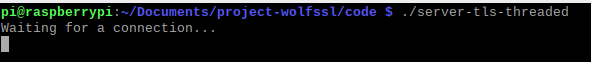
\includegraphics[scale=0.65]{./code/img/1-server.png}
    \caption{Execute WolfSSL server}
    \label{fig:galaxy}
\end{figure}

\begin{figure}[H]
    \centering
    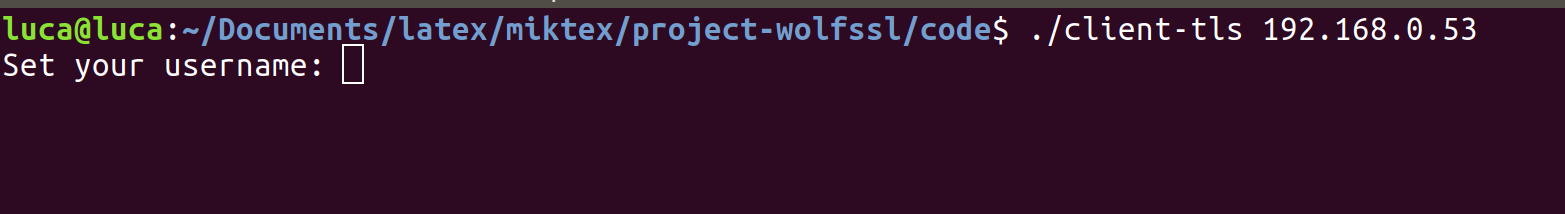
\includegraphics[scale=0.248]{./code/img/1-client.png}
    \caption{Execute WolfSSL client}
    \label{fig:galaxy}
\end{figure}

After the execution of the server, a client can connect to it and the ssl handshake starts.
\\With the hello packet below, the client provides an ordered list of 27 cipher suites that it will support for encryption. The list is in the order preferred by the client, with highest preference first. This list can be modified by the programmer.
\\In this case, the client provides a list of optional extension which the server can use to take action or enable new features, for example:
\begin{itemize}
\item key\_share 
\begin{itemize}
\item the client sends one or more public keys using an algorithm that it thinks the server will support. This allows the rest of the handshake after the ClientHello message to be encrypted.
\end{itemize}
\item supported\_version
\begin{itemize}
\item the client indicates its support of TLS 1.3
\end{itemize}
\end{itemize}
\begin{figure}[H]
    \centering
    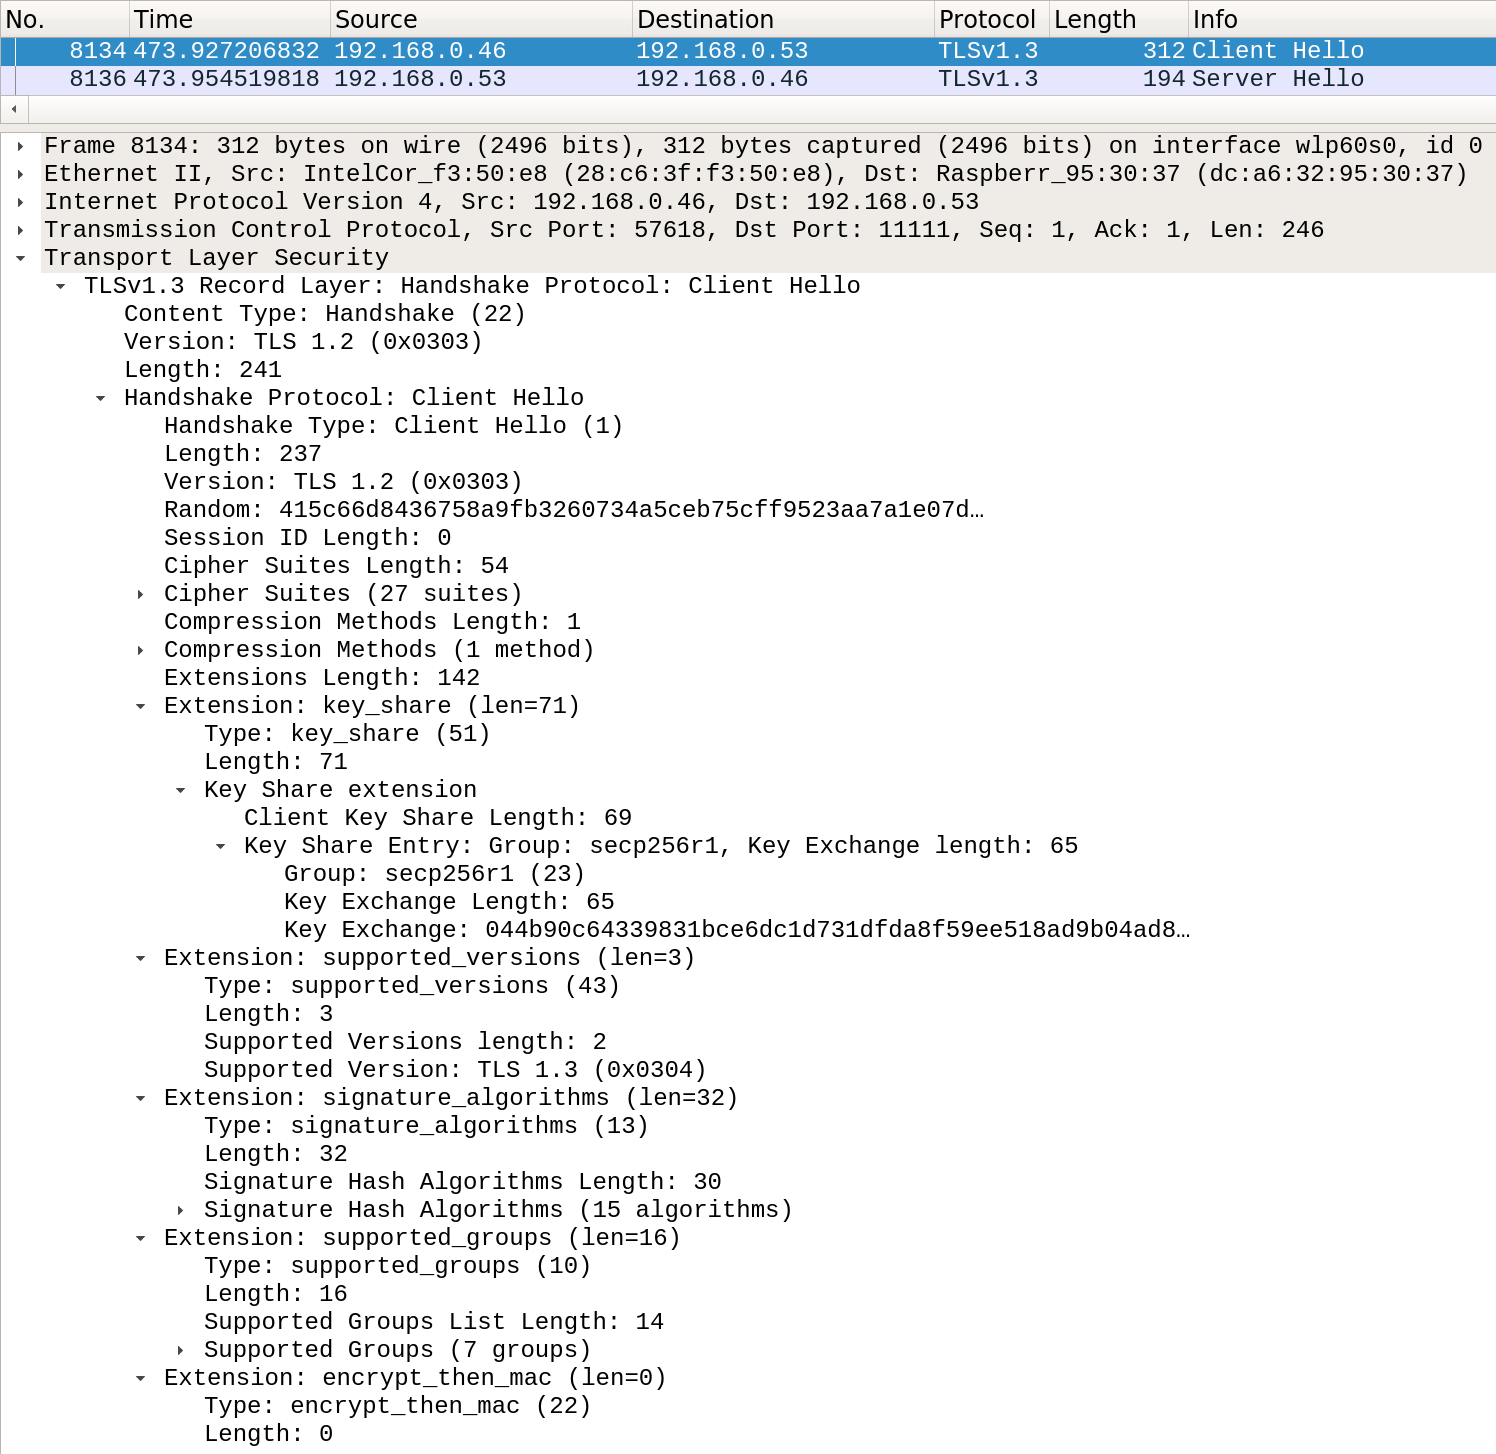
\includegraphics[scale=0.248]{./code/img/client-hello.png}
    \caption{Client Hello}
    \label{fig:galaxy}
\end{figure}


In the Server Hello packet, the server has selected cipher suite 0x1301 (TLS\_AES\_128\_GCM\_SHA256) from the list of options given by the client.
\\The server sends also a public key using the algorithm of the public key sent by the client. Once this is sent encryption keys can be calculated and the rest of the handshake will be encrypted.
The rest of the packets are encrypted. 

\begin{figure}[H]
    \centering
    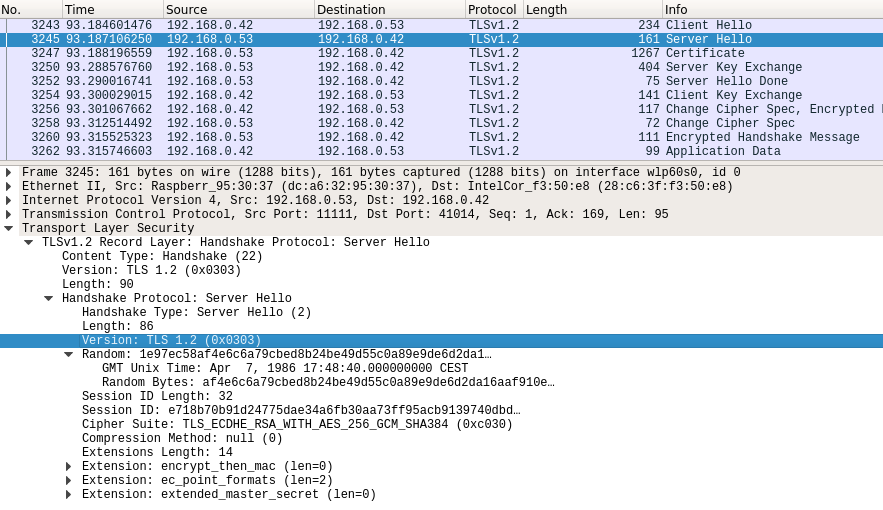
\includegraphics[scale=0.248]{./code/img/server-hello.png}
    \caption{Server Hello}
    \label{fig:galaxy}
\end{figure}
\pagebreak

After the SSL handshake the situation in the server GUI is:
\begin{figure}[H]
    \centering
    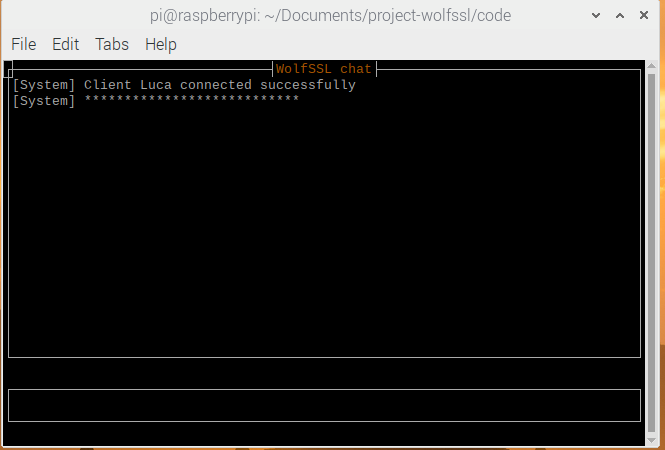
\includegraphics[scale=0.6]{./code/img/2-server.png}
    \caption{Client connected, server GUI}
    \label{fig:galaxy}
\end{figure}

\pagebreak
To test the exact function of the programs, I sent several messages between the laptop and the raspberry:
\begin{figure}[H]
    \centering
    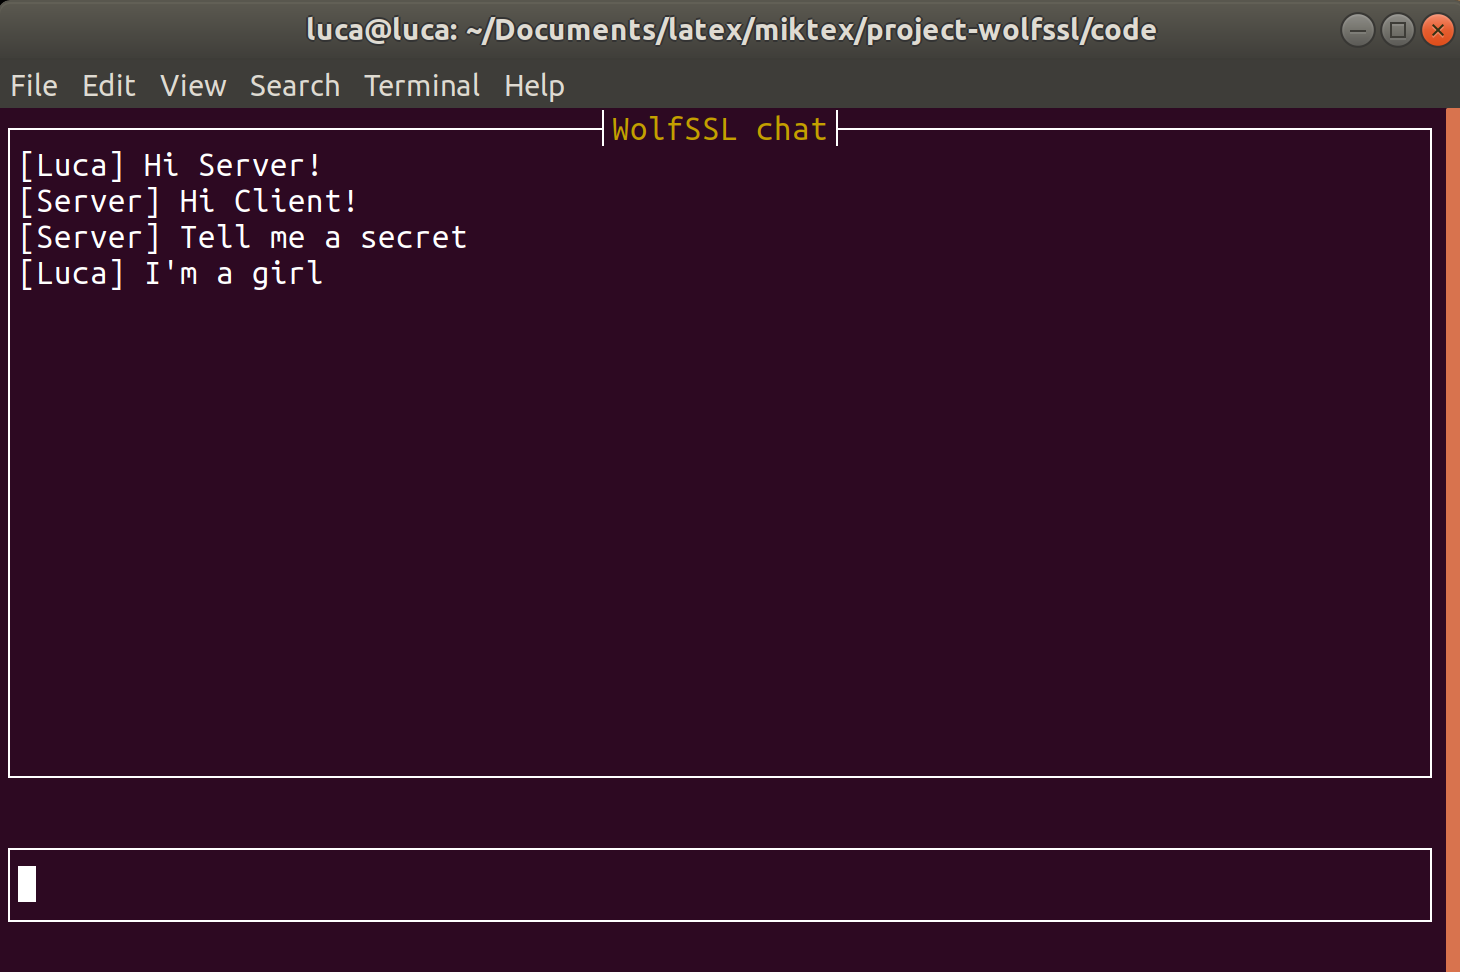
\includegraphics[scale=0.20]{./code/img/2-client.png}
    \caption{Exchange messages. Client side}
    \label{fig:galaxy}
\end{figure}
\begin{figure}[H]
    \centering
    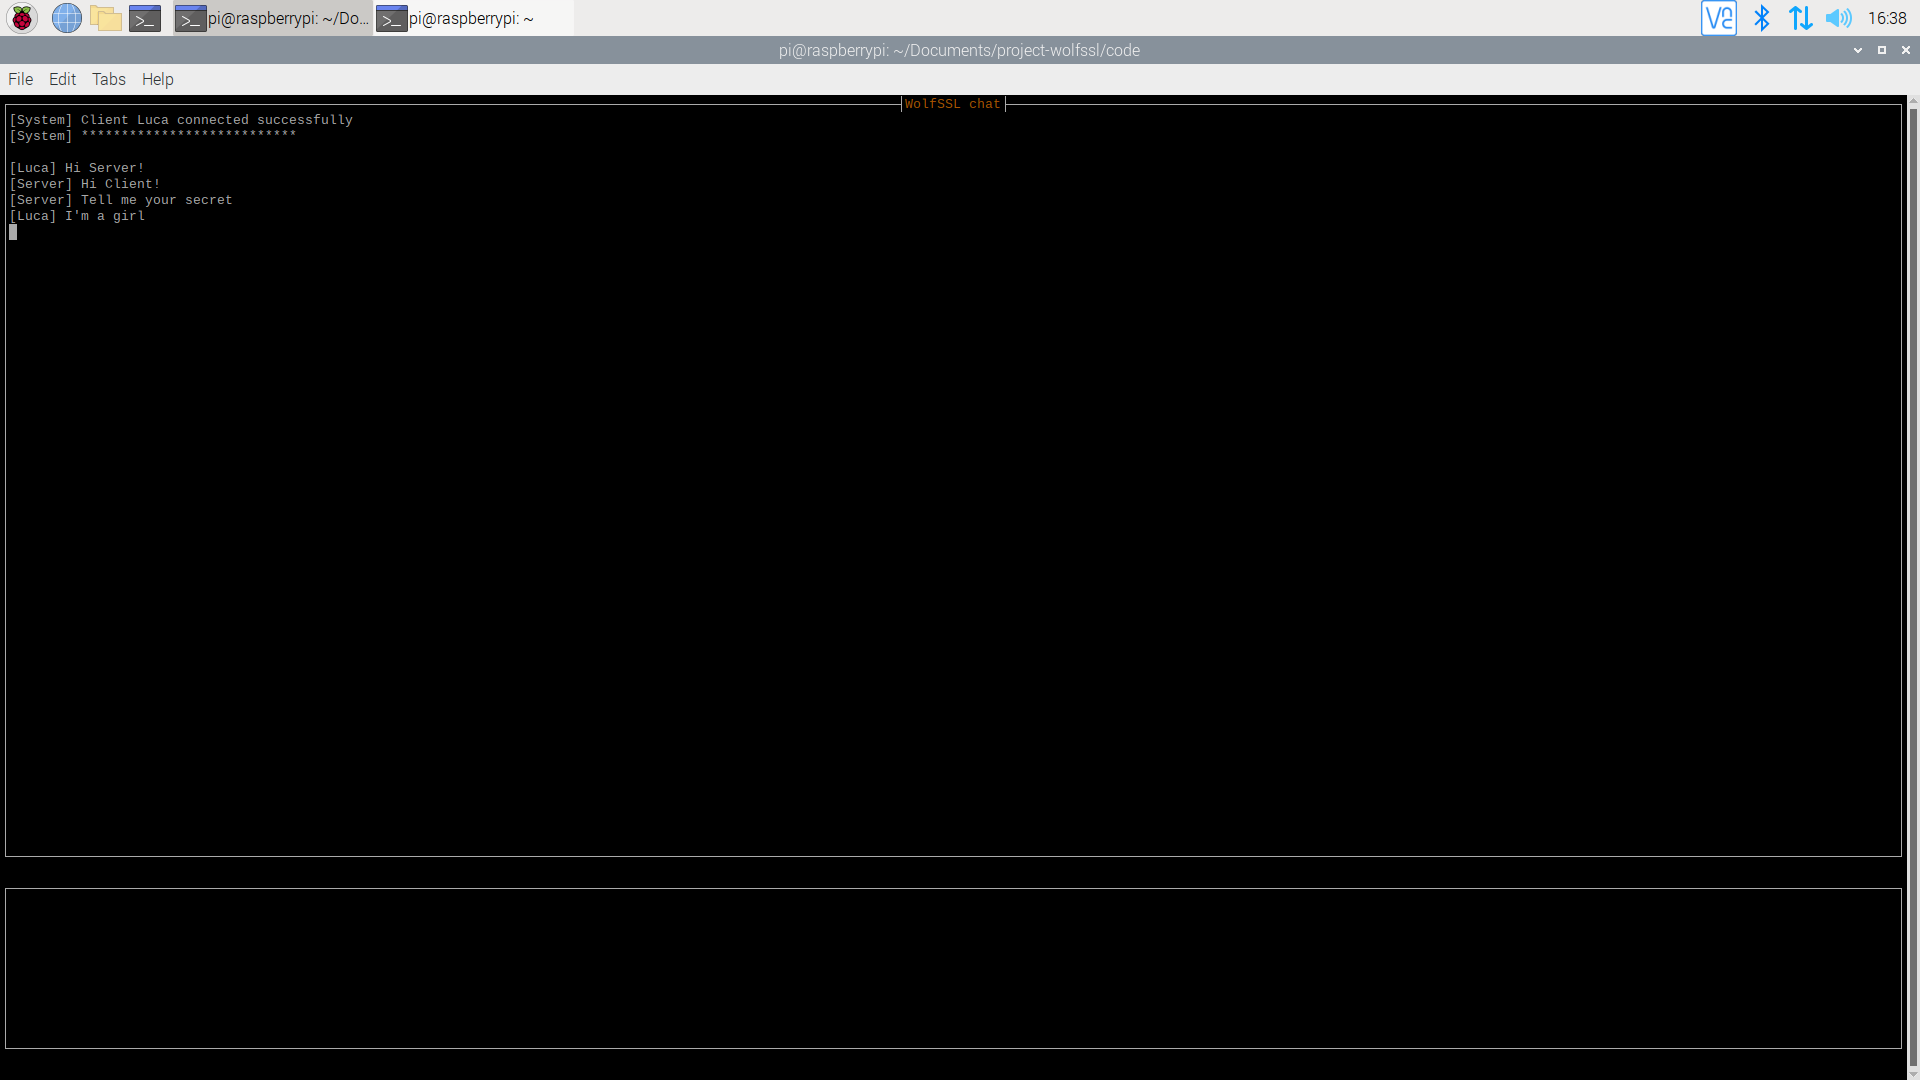
\includegraphics[scale=0.44]{./code/img/3-server.png}
    \caption{Exchange messages. Server side}
    \label{fig:galaxy}
\end{figure}
\pagebreak

As you can see, the messages are encrypted.
\begin{figure}[H]
    \centering
    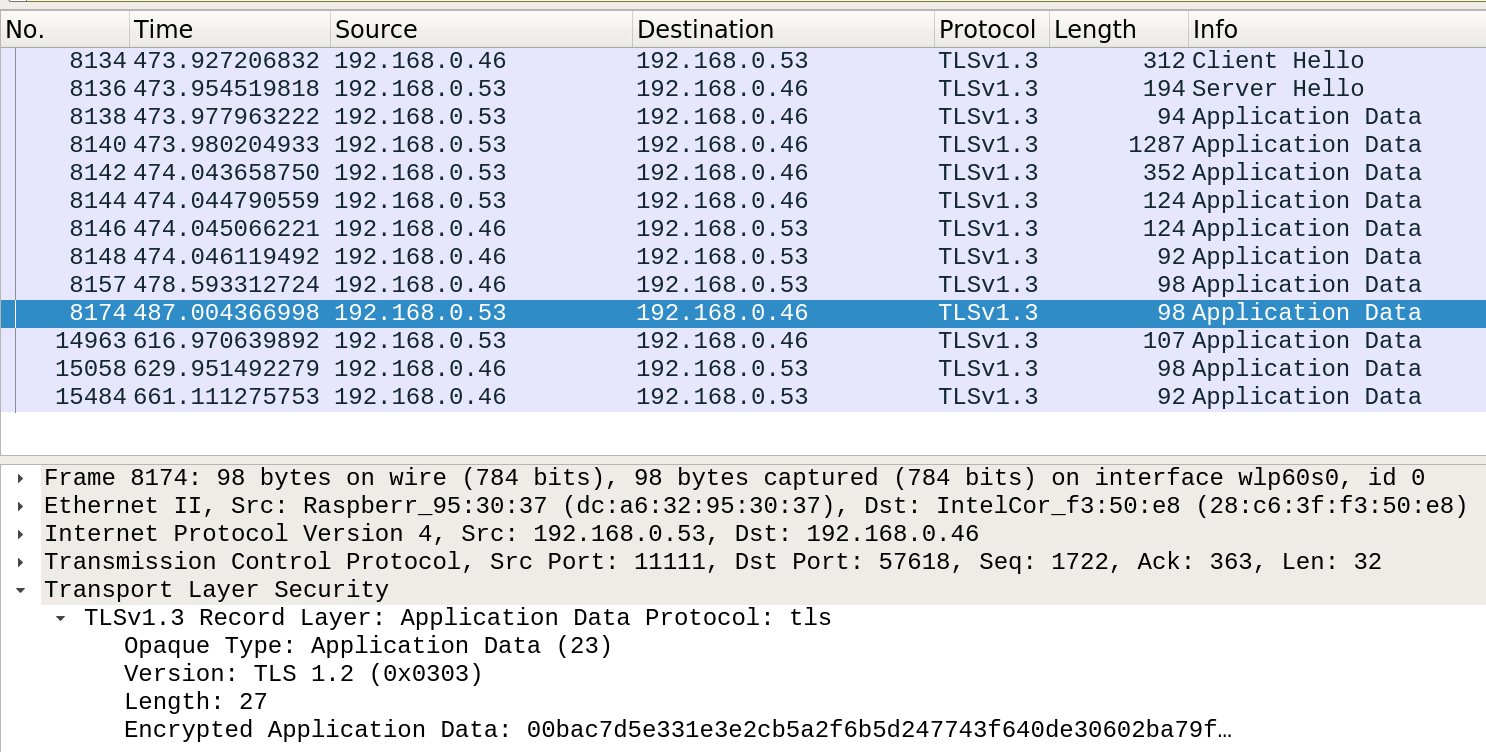
\includegraphics[scale=0.248]{./code/img/application_data.png}
    \caption{Application data}
    \label{fig:galaxy}
\end{figure}
\pagebreak
These are the end of communication screens from the client and from the server:
\begin{figure}[H]
    \centering
    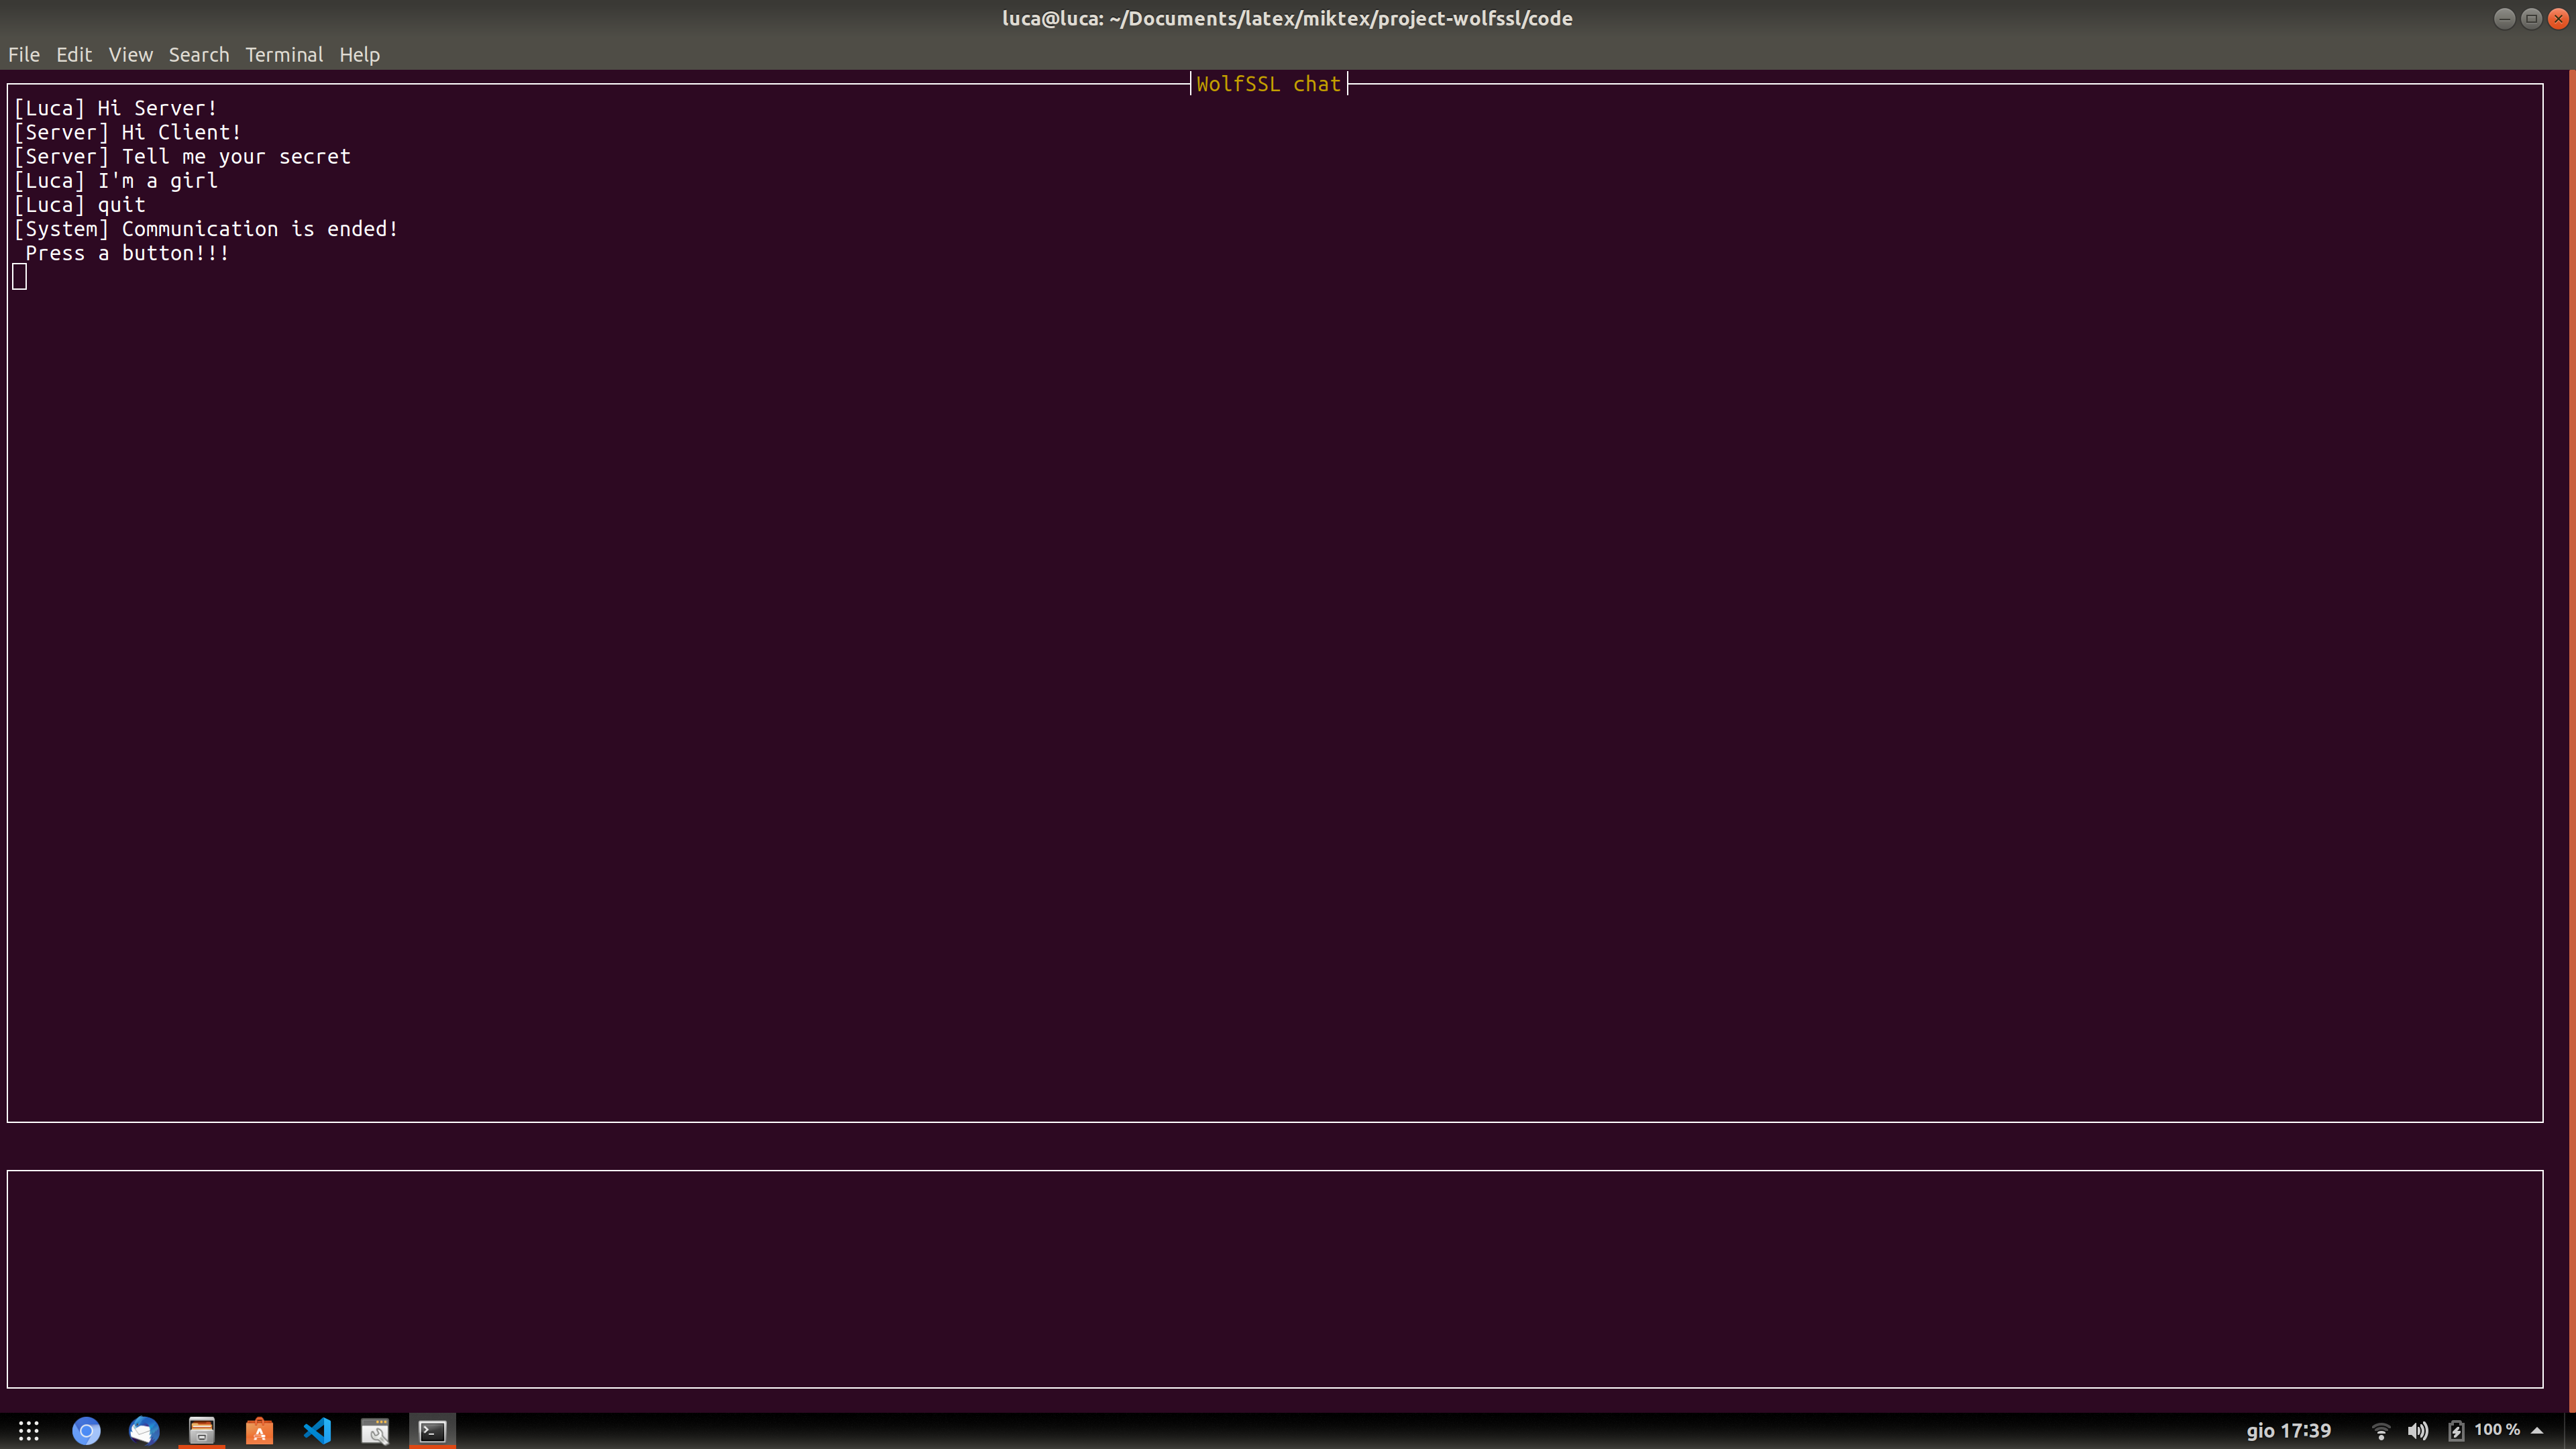
\includegraphics[scale=0.2]{./code/img/3-client.png}
    \caption{Execute WolfSSL client}
    \label{fig:galaxy}
\end{figure}
\begin{figure}[H]
    \centering
    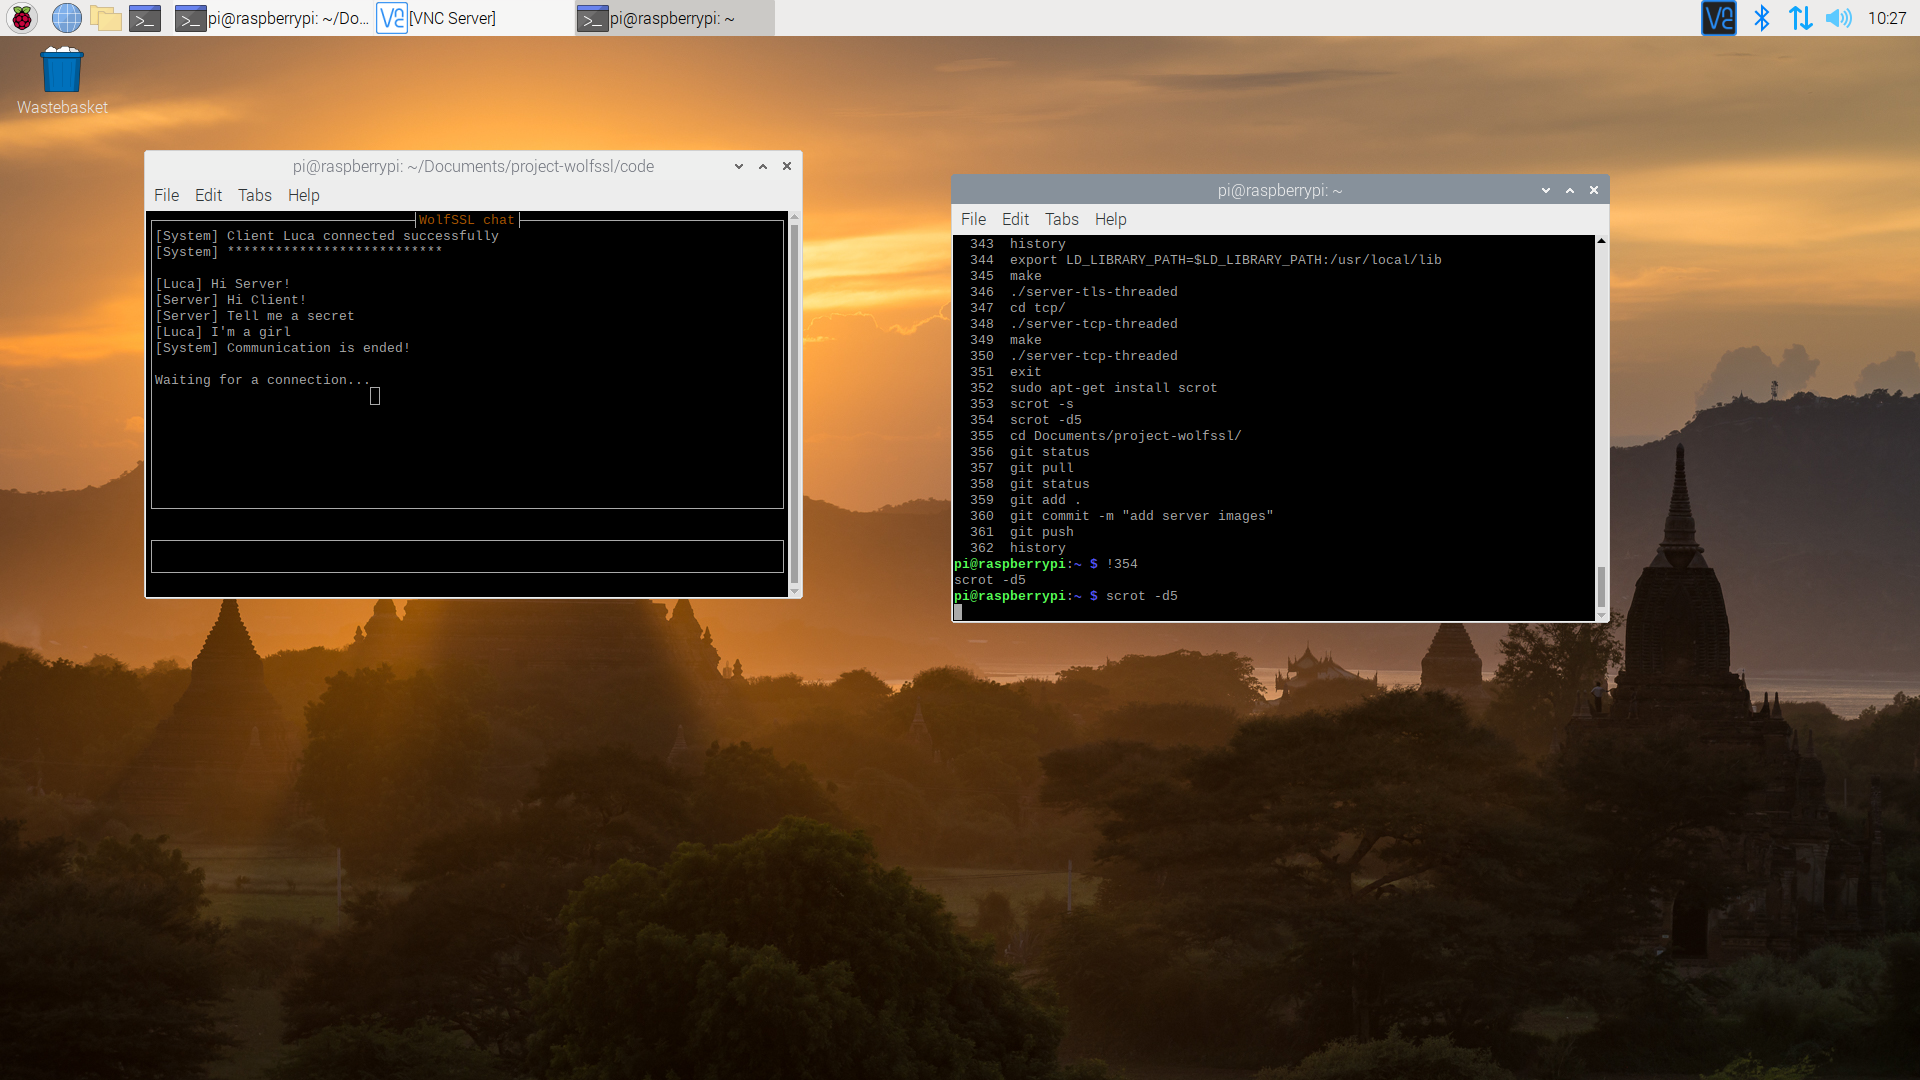
\includegraphics[scale=0.45]{./code/img/4-server.png}
    \caption{Execute WolfSSL client}
    \label{fig:galaxy}
\end{figure}


************ServerKeyExchange has been removed in TLS 1.3*********

\chapter{Differences between WolfSSL and OpenSSL}
\section{Introduction}

The main differences are:
\begin{itemize}
\item Memory Usage
\begin{itemize}
\item WolfSSL can be up to 20 times smaller than OpenSSL; The build size is between 20 and 100 KB and the runtime memory usage between 1 and 36 KB. This gives a magior advantage of integrating in smaller embedded devices. 
\end{itemize}
\item Hardware Crypto
\begin{itemize}
\item WolfSSL has a partnership with the most MCU manufacturers which allows to be quite early in the market to support hardware acceleration on huge list of platforms.
\end{itemize}
\item Portability
\begin{itemize}
\item WolfSSL is more portable than OpenSSL because is made for real-time, mobile, embedded and enterprise systems.
\end{itemize}
\end{itemize}


\end{document}
